\message{ !name(rapport_monte_carlo.tex)}\documentclass[12pt,a4paper]{article}

\usepackage[utf8]{inputenc}
\usepackage[francais]{babel}
\usepackage[T1]{fontenc}
\usepackage{amsmath}
\usepackage{amsfonts}
\usepackage{amssymb}
\usepackage[colorlinks=false]{hyperref} % liens dans le sommaire
% \usepackage[top = 2.54cm, bottom = 2.54cm, left = 2.54cm, right = 2.54cm]{geometry}
\usepackage[top = 2cm, bottom = 2cm, left = 2cm, right = 2cm]{geometry}
\usepackage{graphicx}
\usepackage{caption}
\hypersetup{colorlinks, linkcolor = black, citecolor = black} % enlève couleur des liens
\usepackage{hyperref}
\usepackage{color}
\frenchbsetup{StandardLists=true}
\usepackage{float}
\usepackage{fancyhdr}
\usepackage{mathtools}
\pagestyle{fancy}

\newcommand{\dx}[1]{\dfrac{\partial #1}{\partial x}}
\newcommand{\norm}[1]{\big|\big|#1\big|\big|}
\newcommand{\question}[2]{\paragraph{Question #1 --}\hspace{-7pt}\textit{#2} \\}
\newcommand{\tphi}{\widetilde{\Phi}}
\newcommand{\intsigma}{\widetilde{\Sigma}}
\newcommand{\F}{\mathcal{F}}
\begin{document}

\message{ !name(rapport_monte_carlo.tex) !offset(-3) }


\begin{titlepage}
  ~\vspace{90pt}
  \centering \bfseries

  \huge Rapport de TP \\AMS302

  \vspace{50pt}
  \rule{0.5\textwidth}{1pt}
  \vspace{50pt}

  \Huge Solveur Monte-Carlo \\ pour le transport de particules neutres

  \vspace{50pt}
  \rule{0.5\textwidth}{1pt}

  \vspace{50pt}
  \huge {\itshape Benoît Sohet \\ \& \\ Aurélien Valade}

  \vfill
  \begin{tabular}{cc}
    \begin{minipage}{.49\textwidth}
      \centering
      \includegraphics[height=0.1\textheight]{logo_ups}
    \end{minipage}
    &
      \begin{minipage}{.49\textwidth}
        \centering
        \includegraphics[height=0.1\textheight]{logo_ensta}
      \end{minipage}
  \end{tabular}

\end{titlepage}

\newpage

\section{Introduction}

Dans ce TP on cherche à résoudre le problème différentiel suivant 
\begin{equation}
  \label{eq:principal}
  \begin{cases}
    \mu \dx{\Phi}(x, \mu) + \Sigma_t \Phi(x, \mu) =
    \dfrac{1}{2} \Sigma_s(x) \int_1^{-1} \Phi(x, \mu') d\mu' + S(x, \mu) & \forall (x, \mu) \in [0,1]\times[-1,1]  \medskip\\ 
    \mu n(x) < 0  & \forall (x, \mu) \in \{0,1\}\times[-1,1] 
  \end{cases}
\end{equation}

\begin{itemize}
\item $\Phi(x, \mu)$ le flux neutronique
\item $\Sigma_t$ la section efficace totale 
\item $n(x)$ la normale sortante : $n(0) = -1, ~ n(1) = 1$
\end{itemize}

On fixe pour cela deux types de conditions aux limites 
\begin{itemize}
\item Flux entrant à gauche
  \begin{equation}
    \begin{cases}
      \Phi^{-} (0, \mu) = \frac{1}{\mu}  ~~~ \forall \mu \in [0,1]\\
      \Phi^{-} (1, \mu) = 0 ~~~ \forall \mu \in [-1,0]
    \end{cases}
  \end{equation}
\item Source nulle ou unitaire
  \begin{align}
    S(x) &= 0 ~~~ \forall x \in [0,1] \\
    S(x) &= 1 ~~~ \forall x \in [0,1] 
  \end{align}
\end{itemize}	

On utilisera dans la suite l'erreur pour une fonction $f$ et son approximation $\tilde{f}$ : 
\begin{equation}
  e_{L_2}(f, \tilde{f}) = \frac{\norm{f-\tilde{f}}_{L_2}}{\norm{f}_{L_2}}
\end{equation}

\question{1}{Quelle est la densité de probabilité du libre parcours d'un neutron dans un matériau de section
  efficace totale $\Sigma$ ? Comment échantillonner une variable aléatoire suivant cette loi ?}
\subparagraph{Densité \textit{p} :} Nous allons d'abord calculer la fonction de répartition correspondant :
\begin{equation}
  F(l)=\int_a^{a+l} p(x) dx ,
\end{equation}
(avec $a$ une constante quelconque), puis on déduira :
\begin{equation}
  p(l)=\left\|\frac{\partial F}{\partial l}\left(l\right)\right\| .
\end{equation}

$F(l)$ est la probabilité qu'un neutron n'ait pas intéragi (ni absorption ni diffusion) lors d'un parcours de longueur $l$ selon l'axe $(0x)$, autrement dit la probabilité que ce neutron ait un libre parcours de longueur $\frac{l}{\mu}$.

Or, la probabilité qu'il n'y ait pas d'intéraction sur une longueur infinitésimal $\delta l$ est :
\begin{equation}
  1- \frac{\Sigma_t}{\mu} \delta l .
\end{equation}

Il suffit alors de multiplier cette expression autant de fois qu'il y a $\delta l$ dans $l$, c'est-à-dire $N=\frac{l}{\delta l}$, pour parvenir à $F(l)$, puisqu'on peut considérer ces évènements comme indépendants : 
\begin{equation}
  \left(1-\frac{\Sigma_t}{\mu} \delta l\right)^N = \left(1-\frac{\Sigma_t}{\mu} \frac{l}{N}\right)^N  \xrightarrow[N \rightarrow \infty]{} e^{-\frac{\Sigma_t}{\mu} l} .
\end{equation}

De là, la probabilité $p(l) dl$ d'interaction entre $l$ et $l+dl$ (sachant qu'il n'y en a pas eu jusqu'à présent) vaut :

\begin{equation}
  p(l) dl = \frac{\Sigma_t}{\mu} e^{-\frac{\Sigma_t}{\mu} l} dl .
\end{equation}

\subparagraph{Échantillonnage :}

Pour reproduire cette densité de probabilité numériquement par une variable aléatoire $X$, il suffit d'expliciter $F^{-1}$, car :
\begin{equation}
  P(a\leq X\leq b) {\color{red}=} F(b) - F(a) {\color{red}=} P(F(a)\leq U\leq F(b)) {\color{red}=} P(a\leq F^{-1}(U)\leq b) ,
\end{equation}

où $U$ est une variable aléatoire uniforme. Or :

\begin{equation}
  F^{-1}(y) = -\frac{\mu}{\Sigma_t} \log(y) .
\end{equation}

Il suffit donc d'utiliser une fonction \textit{random} numérique à valeurs dans l'image de la fonction de répartition $F$, $[0;1]$, puis d'appliquer l'inverse de cette fonction, $F^{-1}$.
On obtient ainsi la variable aléatoire suivant la loi $p(l) dl$.

\subparagraph{Remarque :} Lorsque $\mu<0$, $dl<0$ et $N<0$, mais dans chaque formule se fait le produit (ou le rapport) de deux de ces quantités, ce qui redevient alors positif.

\question{2}{Connaissant les trajectoires (marches aléatoires) d'une population neutronique, comment construire un estimateur du flux neutronique?}

Le flux neutronique en $x$ d'une population de neutrons est par définition le nombre de ces neutrons dont la trajectoire s'est arrêtée en $x$ (c'est-à-dire lorsqu'il y a eu interaction).

\section{Matériau purement absorbant}

\subsection{Matériau homogène - source ponctuelle}

\question{3}{Trouver la solution analytique au problème \autoref{eq:principal} avec les conditions suivantes :}

\begin{equation}
  \Sigma_s=0, ~~~ \dx{\Sigma_t} = 0, ~~~ S(x, \mu) = \delta(x)
\end{equation}
On a donc 
\begin{equation}
  \dx{\Phi} + \frac{\Sigma_t}{\mu} \Phi = \frac{1}{\mu} \delta(x)
\end{equation}

Une fois soumis à la transformée de Fourrier on a 
\begin{align}
  &i \omega \tphi + \frac{\Sigma_t}{\mu} \tphi = \frac{1}{\mu} \\
  &\tphi = -\frac{i}{\mu\left(\omega - \frac{i \Sigma_t}{\mu}\right)}
\end{align}
on peut donc écrire 
\begin{equation}
  \Phi (x, \mu) = -\frac{i}{2\pi\mu} \int_{\mathbb{R}} \frac{e^{i\omega x}}{\omega - \frac{i \Sigma_t}{\mu}} d\omega 
\end{equation}
or d'après le théorème des résidus appliqué sur le contour fermé autour du point singulier $\omega = i\frac{\Sigma_t}{\mu}$
\begin{equation}
  \gamma_r = [-r,r]\cup\left\{r e^{-i \theta}, \theta \in [0, \pi] \right\} ~~~ \mbox{avec } r \to \infty
\end{equation}
on trouve que
\begin{align}
  \Phi (x, \mu) &= - (2 \pi i) \frac{i}{2\pi\mu} e^{i \frac{i \Sigma_t}{\mu} x} \\
                &= \frac{1}{\mu} e^{-\frac{\Sigma_t}{\mu} x} 
\end{align}

Ces fonctions sont représentés dans la \autoref{fig:delta_many_mu}.

\begin{figure}[h]
  \centering
  \includegraphics[height=.4\textheight]{Code/phi_source_delta_many_mu}
  \caption{Fonctions $\Phi$ pour différent $\mu$.}
  \label{fig:delta_many_mu}
\end{figure}

\question{4}{Implémenter le code Monte-Carlo pour ce modèle}

Cf code commenté.

\begin{figure}[h]
  \centering
  \includegraphics[height=0.3\textheight]{Code/phi_sigma_cst_source_delta}
  \includegraphics[height=0.3\textheight]{Code/phi_sigma_cst_source_cste}
  \includegraphics[height=0.3\textheight]{Code/phi_sigma_cst_source_cste_mu_neg}
  \caption{Courbes théoriques et résultats des simuluations Monte Carlo pour différents cas de figure.
    Haut : source ponctuelle en 0 avec $\mu=0.5$ et $\Sigma_t=2$ pour $10^6$ particules avec une erreur $e_{L_2} = 3\,10^{-6}$. 18260 particules sont sorties du segment unitaire par la droite. 
    Milieu : source constante sur $[0,1]$ avec $\mu=0.5$ et $\Sigma_t=3$ pour $10^6$ particules avec une erreur $e_{L_2} = 3\,10^{-6}$.
    Bas :  source constante sur $[0,1]$ avec $\mu=-0.5$ et $\Sigma_t=3$ pour $10^6$ particules avec une erreur $e_{L_2} = 3\,10^{-6}$.}
  \label{fig:sigmacst}
\end{figure}

\subsection{Matériau homogène - source uniforme}

\question{5}{Trouver la solution analytique au problème \autoref{eq:principal} avec les conditions suivantes :}

\begin{equation}
  \Sigma_s=0, ~~~ \dx{\Sigma_t} = 0, ~~~ S(x, \mu) = 1
\end{equation}
On a donc en considérant un flux entrant nul à gauche 
\begin{gather}
  \dx{\Phi} + \frac{\Sigma_t}{\mu} \Phi = \frac{1}{\mu} \\
  \begin{cases}
    \Phi(x, \mu)= \frac{1}{\Sigma_t}\left( 1-e^{-\frac{\Sigma_t}{\mu}x}\right) &~~~ \mbox{si } \mu>0 \medskip \\ %\frac{1}{\mu}e^{-\frac{\Sigma_t}{\mu}x} +
    \Phi(x, \mu)= \frac{1}{\Sigma_t}\left( 1-e^{-\frac{\Sigma_t}{\mu}(x-1)}\right) &~~~ \mbox{si } \mu<0 
  \end{cases}
\end{gather}

\begin{figure}[h]
  \centering
  \includegraphics[height=.4\textheight]{Code/phi_source_cste_many_mu}
  \caption{Fonctions $\Phi$ pour différent $\mu$.}
  \label{fig:cste_many_mu}
\end{figure}

\subsection{Matériau hétérogène - source ponctuelle}

\question{6}{Trouver la solution analytique au problème \autoref{eq:principal} avec les conditions suivantes :}

\begin{equation}
  \Sigma_s=0, ~~~
  \Sigma_t =
  \begin{cases}
    1 &\mbox{si } x<0.3 \\
    3 &\mbox{si } 0.3<x<0.7 \\
    1 &\mbox{si } 0.7<x \\
  \end{cases}
  , ~~~ S(x, \mu) = \delta(x)
\end{equation}

On pose l'intégrale continue de $\Sigma_t(x)$ 
\begin{equation}
  \intsigma(x) =
  \begin{cases}
    x &\mbox{si } x<0.3 \\
    3(x-0.3)+0.3 &\mbox{si } 0.3<x<0.7 \\
    (x-0.7)+1.5 &\mbox{si } 0.7<x \\
  \end{cases}
\end{equation}

On résout sur l'intervale $x\in[0,0.3]$ comme dans la question 3 :
\begin{equation}
  \Phi(x, \mu) = \frac{1}{\mu} e^{-\frac{\Sigma_t x)}{\mu}} ~~~ \mbox{si } x<0.3
\end{equation}
et on prolonge sur tout le segment grâce à $\intsigma(x)$ 
\begin{equation}
  \Phi(x, \mu) = \frac{1}{\mu} e^{-\frac{\intsigma(x)}{\mu}} 
\end{equation}
que l'on peut voir représentée en \autoref{fig:phi}.

\begin{figure}[h]
  \centering
  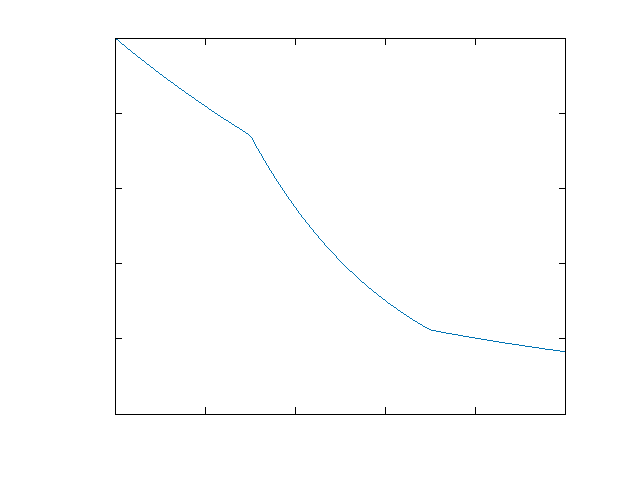
\includegraphics[width=.7\textwidth]{phi}
  \caption{Fonction $\Phi(x, \mu=1)$ pour $\Sigma_t$ variable avec une source ponctuelle en 0.}
  \label{fig:phi}
\end{figure}

On normalise pour obtenir une loi de probabilité
\begin{equation}
  P(x) = \frac{\lambda}{\mu}
  \begin{cases}
    \exp(-x/\mu)         & x<0.3\\
    \exp(-(3x-0.6)/\mu) & 0.3<x<0.7\\
    \exp(-(x+0.8)/\mu)  & 0.7<x
  \end{cases}
\end{equation}
et on y associe une fonction de répartition
\begin{equation}
  \F(x) = \lambda
  \begin{cases}
    C_1 - \exp(-x/\mu)             & x<0.3\\    
    C_2 - 1/3 \exp(-(3x-0.6)/\mu) & 0.3<x<0.7\\
    C_3 - \exp(-(x+0.8)/\mu)      & 0.7<x      
  \end{cases}
\end{equation}
avec
\begin{align}
  &C_1 = 1 && \F(0)=0 \\
  &C_2 = 1 - 2/3 \exp(0.3/\mu) && \mbox{continuité en }x=0.3 \\
  &C_3 = C_2 + 2/3 \exp(-1.5/\mu) &&  \mbox{continuité en }x=0.7 \\
  &\lambda = 1/C_3 &&  \F(x)  \xrightarrow[x \to \infty]{} 1
\end{align}

\textbf{Attention : } ce raisonnement ne fonctionne que pour des particules partant de $x=0$ ! La loi de probabilité d'aller à une distance $x$ a une toute autre forme si la source est quelconque.

\question{7}{Implémenter un solveur Monte-Carlo utilisant la méthode de Woodcock pour échantillonner le libre parcours de neutrons dans un tel matériau. On fournira les mêmes résultats que pour la question 4.}

\begin{figure}[h]
  \centering
  \includegraphics[height=.4\textheight]{Code/sigmavar}
  \caption{Courbe théorique et points expérimentaux pour $\Phi(x,\mu = 0.7)$, avec une erreur $e_{L_2}=2\,10^{-4}$.}
  \label{fig:sigmavar}
\end{figure}

Cependant, la méthode employée est très différente de celle employée pour les questions précédentes. En effet, on trouve une correlation entre une quantité proportionelle à $\Phi$ et le résultat du Monte-Carlo, mais il ne s'agit de $\Phi$ qu'à une fonction de $\mu$ près. La méthode de dénombrement employée pour trouver le résultat présenté en \autoref{fig:sigmavar} ne compte que les particules arrivées en $x$ et non l'ensemble des particules ayant traversé $x$ car cette méthode a priori correcte amène à trouver l'intégrale de $\Phi$, comme présenté en \autoref{fig:pb}. Un facteur 3 entre la courbe dérivée du Monte-Carlo et la courbe de $\Phi$ pourrait être corrélée avec la valeur maximale de $\Sigma$. 

\begin{figure}[h]
  \centering
  \includegraphics[height=.3\textheight]{Code/theo} \\
  \includegraphics[height=.3\textheight]{Code/dmc} \\
  \includegraphics[height=.3\textheight]{Code/mc} 
  \caption{Courbes mettant en valeur la relation dérivée--intégrale entre la solution théorique et le résultat du Monte Carlo. Haut : courbe théorique ; Milieu : dérivée du Monte-Carlo ; Bas : Monte-Carlo.}
  \label{fig:pb}
\end{figure}

\end{document}

%%% Local Variables:
%%% mode: latex
%%% TeX-master: t
%%% End:

\message{ !name(rapport_monte_carlo.tex) !offset(-337) }
